\chapter{Appendix}
\section{Probability Theory}
\begin{lemma}\leavevmode \label{appx1}
    \begin{enumerate}[label=(\roman*), font=\normalfont]
        \item\label{appx1:i} \(\Pr(A\cap B\mid C) = \Pr(A \mid B \cap C)\Pr(B\mid C) \)
        \item\label{appx1:ii} \(\Pr(A\mid C)=\sum\limits_{n\in\N} \Pr(A \mid B_n \cap C)\Pr(B_n\mid C)  \)
        for  \(\Pr\left(\biguplus_{n\in\N}B_n\right)=1 \)
        \item\label{appx1:iii} \(\E[X\mid C]=\sum\limits_{n\in\N} \E[X\mid C \cap B_n] \Pr(B_n \mid C) \) for  \(\Pr\left(\biguplus_{n\in\N}B_n\right)=1 \)
    \end{enumerate}
\end{lemma}
\begin{proof}
    \ref{appx1:i}
    \[
        \Pr(A\cap B\mid C)
        =\frac{\Pr(A\cap B\cap C)}{\Pr(B\cap C)}\frac{\Pr(B\cap C)}{\Pr(C)}
        =\Pr(A\mid B\cap C)\Pr(B\mid C)
    \]
    \ref{appx1:ii}
    \begin{align*}
        \Pr(A\mid C)&=\Pr\left(A\cap \biguplus_{n\in\N} B_n \;\middle|\; C\right)
        =\sum_{n\in\N} \Pr(A\cap B_n\mid C)\\
        &\lxeq{\text{\ref{appx1:i}}} \sum_{n\in\N} \Pr(A \mid B_n \cap C)\Pr(B_n\mid C)
    \end{align*}
    \ref{appx1:iii}
    \begin{align*}
        \E[X\mid C]
        &=\frac{1}{\Pr(C)} \int_C X d\Pr 
        \xeq{(*)}\sum_{n\in\N}\frac{1}{\Pr(C)} \int_{C\cap B_n} X d\Pr\\
        &=\sum_{n\in\N} \frac{\Pr(C\cap B_n)}{\Pr(C)} \frac{1}{\Pr(C\cap B_n)} 
        \int_{C\cap B_n} X d\Pr \\
        &=\sum_{n\in\N}\E[X\mid C\cap B_n]\Pr(B_n\mid C) \qedhere
    \end{align*}

\end{proof}
\begin{lemma}\label{appx2}
    Let \((\Omega,\cA,\mu)\) be a measure space and a function \(f\) exists with
    \begin{align*}
        &f\colon \Omega \to \R \text{ injective and measureable,} \\
        &f^{-1}\colon f(\Omega)\to \Omega \text{ measureable.}
    \end{align*}
    Then for \(X\) \(\Omega\)-valued random variable and
    \(Y\) \(f(\Omega)\)-valued random variable
    \[
        \Pr_{f\circ X} =\Pr_Y \iff \Pr_X=\Pr_{f^{-1}\circ Y}
    \]
\end{lemma}
\begin{proof}
    ``\(\Leftarrow\)'' Let \(A\in\cB(\R)\), then w.l.o.g. \(A\subseteq f(\Omega)\) otherwise
    \[
        \Pr_{f\circ X}(A)=\Pr(A\cap f(\Omega))+\underbracket[0.7pt]{
            \Pr_{f\circ X}(A\cap f(\Omega)^\complement)
            }_{=0}=\dotsc=\Pr_Y(A) 
    \]
    Thus \(f\circ f^{-1}(A)=A\) holds, which finishes this direction with
    \begin{align*}
        \Pr_{f\circ X}(A)
        &=\Pr(X^{-1}\circ f^{-1}(A))=\Pr_X(f^{-1}(A))\\
        &=Pr_{f^{-1}\circ Y}(f^{-1}(A))=\Pr(Y^{-1}\circ f\circ f^{-1}(A))\\
        &=\Pr_Y(A)
    \end{align*}
    ``\(\Rightarrow\)'' Let \(A\in\cA\), then
    \begin{align*}
        \Pr_X(A)&=\Pr(X^{-1}\circ f^{-1}\circ f(A))=\Pr_{f\circ X}(f(A))\\
        &=\Pr_Y(f(A))=\Pr(Y^{-1}\circ f(A))\\
        &=\Pr_{f^{-1}\circ Y}(A) \qedhere
    \end{align*}
\end{proof}
\begin{definition}[Pseudo-inverse]\label{appx3}
    Let \(F\) be a cumulative distribution function, then 
    \[F^\leftarrow (y) \coloneqq \inf\{x\in\R : F(x)\ge y \}\]
    is called the \emph{Pseudo-inverse} of \(F\).
\end{definition}
\begin{lemma}\label{appx pseudo inv distribution}
    Let \(F\) be a cdf, then
    \begin{enumerate}[label=(\roman*), font=\normalfont]
        \item\label{appx3:i} \(
            F^\leftarrow (y)\le x \iff y \le F(x)
        \)
        \item\label{appx3:ii} \(U\sim\cU(0,1) \implies F^\leftarrow(U) \sim F \)
    \end{enumerate}
\end{lemma}
\begin{proof}
    \ref{appx3:i} ``\(\Rightarrow\)''
    \begin{align*}
        y&\le \inf_{x\in \{z\in\R: F(z)\ge y\}} F(x) 
        \xeq{\substack{
            \text{F right-}\\
            \text{continuous}}
        } F(\inf\{z\in\R: F(z)\ge y\})
        \xeq{\text{def.}} F(F^\leftarrow(y))\\
        &\le F(x)
    \end{align*}
    Where the last inequality follows from the assumption \(F^\leftarrow (y)\le x\) and F being non decreasing.

    \noindent ``\(\Leftarrow\)'' Follows simply from the fact that x is included in the set of the infimum. 
    \begin{align*}
        y\le F(x) \implies F^\leftarrow (y) = \inf\{z\in\R:F(z)\ge y\} \le x
    \end{align*}

    \noindent \ref{appx3:ii} is a simple corollary from \ref{appx3:i}
    \[
        \Pr(F^\leftarrow (U)\le x) 
        \xeq{\text{\ref{appx3:i}}} \Pr(U\le F(x)) = F(x) 
        \qedhere
    \]
\end{proof}

\begin{lemma}\label{appx7}
    Some History is irrelevant, if the entire history is irrelevant or more generally
    \[
        \E[X\mid Z, Y_1,Y_2]=\E[X\mid Z] \implies \E[X\mid Z, Y_1]=\E[X\mid Z]
    \]
    for arbitrary random variables \(X, Z, Y_1, Y_2\) with \(Y_2\) being \(\cY\) valued, where \(\cY\) is countable. This is true in particular for
    \[
        \Pr(A\mid Z, Y_1,Y_2)=\E[\mathbbm{1}_A \mid Z, Y_1,Y_2].
    \]
\end{lemma}
\begin{proof} Due to the same argument as in (\ref{constant expectation})
    \[
        \int_{\{Y=y\}} X d\Pr = \int_{\{Y=y\}} \E[X\mid Y]d\Pr = \E[X\mid Y=y] \Pr(Y=y),
    \]
    we can write
    \[
        \E[X\mid Y=y]=\frac{1}{\Pr(Y=y)}\int_{\{Y=y\}} X d\Pr=\E[X \mid \{Y=y\}]
    \]
    which allows us to apply \ref{appx1} \ref{appx1:iii}:
    \begin{align*}
        &\E[X\mid Z=z, Y_1=y_1]\\
        &\lxeq{\text{\ref{appx1}}}\sum_{y_2\in\cY} \underbracket[0.7pt]{\E[X\mid Z=z, Y_1=y_1, Y_2=y_2]}_{=\E[X\mid Z=z]} \Pr(Y_2=y_2\mid Z=z,Y_1=y_1)\\
        &=\E[X\mid Z=z] \underbracket[0.7pt]{\sum_{y_2\in\cY} \Pr(Y_2=y_2\mid Z=z,Y_1=y_1)}_{=1}\qedhere
    \end{align*}
\end{proof}

\begin{lemma}\label{appx8}
    Let \(((X_t,A_t,R_{t+1}),t\in\N_0)\) be a sequence generated with a stationary behaviour \(\pi\) from an episodic MDP. Then for some \(x\in\cX\)
    \[
        K\coloneqq\min\{k\in\N_0:X_k=x\}
    \]
    marks the first visit to \(x\), and conditional on \(K\) being finite (i.e. conditional on \(\{k\in\N_0:X_k=x\}\neq \emptyset\))
    \[
        \sum_{t=K}^\infty R_{t+1}\;\Big|\; K \sim \sum_{t=0}^\infty R_{t+1} \;\Big|\; X_0=x.
    \]
    I.e. the distribution of the reward after the first visit to \(x\) has the same distribution as the distribution of the reward conditional on the starting state \(x\). 
\end{lemma}
\begin{proof}
    Because of
    \[
        \{K=k\}=\{ X_0\neq x, \dots, X_{k-1}\neq x, X_k=x\},
    \]
    we can show for every measurable function \(f\) and for all \(k\in\N_0\):
    \begin{align*}
        &\E\left[f\left(\sum_{t=K}^\infty R_{t+1}\right)\;\middle|\; K=k\right]\\
        &=\E\left[f\left(\sum_{t=k}^\infty R_{t+1}\right)\;\middle|\; X_0\neq x, \dots, X_{k-1}\neq x, X_k=x\right]\\
        &\lxeq{\text{Markov}} \E\left[f\left(\sum_{t=k}^\infty R_{t+1}\right)\;\middle|\; X_k=x\right]\\
        &\lxeq{\text{stationary}} \E\left[f\left(\sum_{t=0}^\infty R_{t+1}\right)\;\middle|\; X_0=x\right]
    \end{align*}
    Since this is independent of \(k\in \N_0\), we get
    \begin{align*}
        \E\left[f\left(\sum_{t=K}^\infty R_{t+1}\right)\;\middle|\; K\right]
        =\E\left[f\left(\sum_{t=0}^\infty R_{t+1}\right)\;\middle|\; X_0=x\right]
    \end{align*}
    for every measurable \(f\) conditional on \(K\) being finite, which implies the distributions are the same.
\end{proof}

\begin{lemma}\label{appx4} For a real valued random variable \(X\), an arbitrary random vector \(Y\) and \(f\) a measurable real valued function 
    \[
        \textnormal{Var}[X\mid Y]=\min_{f} \E[ (X-f(Y))^2\mid Y]
    \]
\end{lemma}
\begin{proof}
    \begin{align*}
        \E[(X-f(Y))^2\mid Y] &= \E[X^2\mid Y] - \E[2Xf(Y)\mid Y] + \E[f(Y)^2\mid Y]\\
        &=\E[X^2\mid Y] - 2f(Y)\E[X\mid Y] + f(Y)^2
    \end{align*}  
    Fr a fixed \(\omega\), \(f(Y(\omega))\eqqcolon a\) is simply a constant. Therefore we can set the first derivative equal to zero:
    \begin{align*}
        \frac{d}{da} \E[(X-f(Y))^2\mid Y](\omega)= -2\E[X\mid Y](\omega) +2a \xeq{!} 0
    \end{align*}
    Since the second derivative is \(2>0\), \(\E[X\mid Y](\omega) = f(Y(\omega))\) is the unique minimum. Which implies that \(\text{Var}[X\mid Y]\) is the minimum regardless of \(\omega\).
\end{proof}
\begin{lemma}\label{appx1:summing over probabilities}
    For a non-negative discrete random variable \(X\)
    \[
        \sum_{t=1}^\infty \Pr(X\ge t)=\E[X]
    \]
\end{lemma}
\begin{proof}
    \begin{align*}
        \sum_{t=1}^\infty \Pr(X\ge t)
        &=\sum_{t=1}^\infty \sum_{k=t}^\infty \Pr(X=k)\\
        &=\sum_{t=1}^\infty \sum_{k=0}^\infty \mathbbm{1}_{k\ge t} \Pr(X=k)\\
        &\lxeq{\text{Fub.}}\sum_{k=0}^\infty \underbracket[0.7pt]{\sum_{t=1}^k 1}_{=k} \cdot \Pr(X=k)\\
        &=\E[X]\qedhere
    \end{align*}
\end{proof}
\begin{lemma}\label{appx1:repeated conditional expectation}
    For random a random variable \(X\) and random vectors \(Y,Z\),
    \[
        \E[ \E[X\mid Y,Z]\mid Y] = \E[X\mid Y]
    \]
\end{lemma}
\begin{proof} For all \(B\) in the sigma algebra of the target space of \(Y\)
    \begin{align*}
        \int_{\{Y\in B\}} \E[\E[X\mid Y,Z]\mid Y ] d\Pr 
        &= \int_{\{Y\in B\}} \E[X\mid Y,Z]d\Pr\\
        &=\int_{\{Y\in B\}} X d\Pr\\
        &=\int_{\{Y\in B\}} \E[X\mid Y] d\Pr
    \end{align*}
    Since both are functions, this yields our initial claim, since these two properties uniquely define the conditional expectation. 
\end{proof}
\begin{lemma}\label{appx:6}
    \begin{align*}
        \E[X\mid \mathbbm{1}_A]=\E[X\mid A]\mathbbm{1}_A +\E[X\mid A^\complement]\mathbbm{1}_{A^\complement}
    \end{align*}
\end{lemma}
\begin{proof}
    Let \(f(\mathbbm{1}_A)=\E[X\mid \mathbbm{1}_A]\), then for \(B\in\sigma(\mathbbm{1}_A)=\{\emptyset,A,A^\complement,\Omega\}\) we know
    \[
        \int_B X d\Pr =\int_B f(\mathbbm{1}_A)d\Pr.
    \]
    In particular this requires
    \begin{align}\label{constant expectation}
        \int_A X d\Pr = \int_A f(\mathbbm{1}_A)d\Pr = f(1) \Pr(A).
    \end{align}
    Thus we know
    \[
        f(1)=\mfrac{1}{\Pr(A)}\int_A X d\Pr=\E[X\mid A].
    \]
    With similar reasoning for \(A^\complement\), we can prove the original claim:
    \begin{align*}
        \E[X\mid \mathbbm{1}_A]
        &=f(\mathbbm{1}_A)=f(1)\mathbbm{1}_A + f(0)\mathbbm{1}_{A^\complement}\\
        &=\E[X\mid A]\mathbbm{1}_A +\E[X\mid A^\complement]\mathbbm{1}_{A^\complement}. \qedhere
    \end{align*}
\end{proof}

\section{Analysis}
\begin{lemma}\label{appx:analysis 0}
    Let \(0<a_n(\vep)\le a_n(\vep_0)\) for \(n\in\N\) and  \(0<\vep\le \vep_0\), then
    \begin{align*}
        &\sum_{n=1}^\infty a_n(\vep_0) < \infty 
        \quad\text{and}\quad \forall n\in\N: \lim_{\vep\to 0} a_n(\vep)= 0 \\
        &\implies \lim_{\vep\to 0}\sum_{n=1}^\infty a_n(\vep)=0
    \end{align*}
\end{lemma}
\begin{proof}
    Select an arbitrary \(\delta>0\), then there is some \(N\in\N\) such that
    \[
        \sum_{n=N+1}^\infty a_n(\vep_0) < \delta/2
    \]
    and some \(\vep_0>\vep>0\) such that
    \[
        \sum_{n=1}^N a_n(\vep)<\delta/2
    \]
    and thus
    \[
        \sum_{n=1}^\infty a_n(\vep)
        \le \sum_{n=N+1}^\infty a_n(\vep_0) +\sum_{n=1}^N a_n(\vep)<\delta \qedhere
    \]
\end{proof}
\begin{lemma}\label{appx:analysis 1}
    Let \(0<p_n(\vep)\le p_n(\vep_0)\) for \(n\in\N\) and \(0<\vep \le \vep_0\), then
    \begin{align*}
        &\prod_{n=1}^\infty p_n(\vep_0) > 0 
        \quad\text{and}\quad \forall n\in\N: \lim_{\vep\to 0} p_n(\vep)= 1 \\
        &\implies \lim_{\vep\to 0}\prod_{n=1}^\infty p_n(\vep)=1
    \end{align*}
\end{lemma}
\begin{proof}
    Since the logarithm is continuous we get
    \begin{align*}
        &\sum_{n=1}^\infty \log(p_n(\vep_0))>-\infty \quad \text{and}\quad \forall n\in\N: \lim_{\vep\to 0} \log(p_n(\vep))= 0\\
        &\implies \sum_{n=1}^\infty -\log(p_n(\vep_0))<\infty \quad \text{and}\quad \forall n\in\N: \lim_{\vep\to 0} \log(p_n(\vep))= 0\\
        &\lximplies{\text{\ref{appx:analysis 0}}} \lim_{\vep\to 0} 
        \sum_{n=1}^\infty -\log(p_n(\vep)) =0\\
        &\implies \lim_{\vep\to 0}\prod_{n=1}^\infty p_n(\vep)=\exp\left( 
            \lim_{\vep\to 0}\log\left( \prod_{n=1}^\infty p_n(\vep) \right)
        \right)=1\qedhere
    \end{align*}
\end{proof}

\section{Autoencoder}\label{appx:autoencoder}
While an autoencoder is usually implemented as a neuronal net, the fact that it is a neuronal net is not essential. What is essential, is that it consists of two parameterized functions \(g\circ f\), where \(f\) is function from \(\R^n\) to \(\R^k\) with \(n>k\), and \(g\colon \R^k\to\R^n\). The parameters are then adjusted, such that \(g\circ f\) is as close as possible to the identity on \(R^n\). The closeness metric depends on the context. Usually it depends on some average distance metric between input and output of a given dataset (for example a set of pictures). Then the function \(f\) can be used to compress high dimensional data to lower dimensional data, and \(g\) can be used to decompress data.
Here is an example with \(n=7,k=2\):

\def\layersep{2.5cm}

\[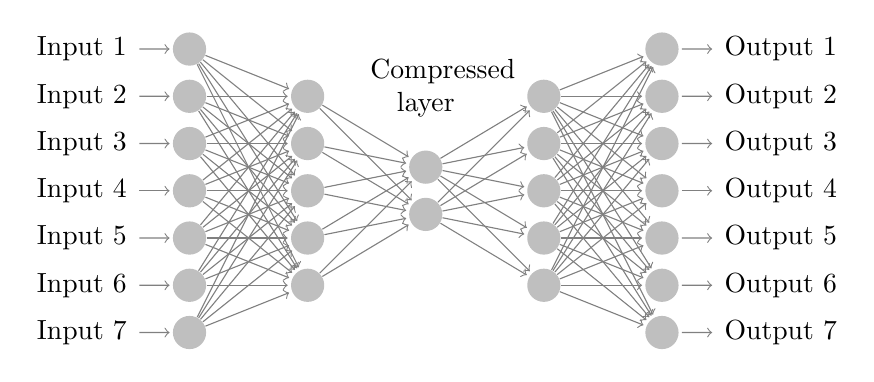
\begin{tikzpicture}[scale=0.6, shorten >=1pt,->,draw=black!50, node distance=\layersep]
    \tikzstyle{every pin edge}=[<-,shorten <=1pt]
    \tikzstyle{neuron}=[circle,fill=black!25,minimum size=12pt,inner sep=0pt]
    \tikzstyle{annot} = [text width=4em, text centered]

    % Draw the input layer nodes
    \foreach \name / \y in {1,...,7}
    % This is the same as writing \foreach \name / \y in {1/1,2/2,3/3,4/4}
        \node[neuron, pin=left:Input \y] (I-\name) at (0,4-\y) {};

    % Draw the hidden layer 1 nodes
    \foreach \name / \y in {1,...,5}
        \node[neuron] (H1-\name) at (\layersep,3-\y) {};

    % Draw the hidden layer 2 nodes
    \foreach \name / \y in {1,...,2}
        \node[neuron] (H2-\name) at (2*\layersep,1.5-\y) {};
    
    % Draw the hidden layer 3 nodes
    \foreach \name / \y in {1,...,5}
        \node[neuron] (H3-\name) at (3*\layersep,3-\y) {};

    % Draw the output layer nodes
    \foreach \name / \y in {1,...,7}
        \node[neuron,pin={[pin edge={->}]right:Output \y}] (O-\name) at (4*\layersep,4-\y) {};

    % Connect every node in the input layer with every node in the
    % hidden layer 1.
    \foreach \source in {1,...,7}
        \foreach \dest in {1,...,5}
            \path (I-\source) edge (H1-\dest);
    
    % Connect every node in the hidden layer 1 with every node in the
    % hidden layer 2.
    \foreach \source in {1,...,5}
        \foreach \dest in {1,...,2}
            \path (H1-\source) edge (H2-\dest);

    % Connect every node in the hidden layer 2 with every node in the
    % hidden layer 3.
    \foreach \source in {1,...,2}
        \foreach \dest in {1,...,5}
            \path (H2-\source) edge (H3-\dest);
        
    % Connect every node in the hidden layer 3 with the output layer
    \foreach \source in {1,...,5}
        \foreach \dest in {1,...,7}
        \path (H3-\source) edge (O-\dest);

    % Annotate the layers
    \node[annot,above of=H2-1, node distance=1cm] {Compressed layer}; 
\end{tikzpicture}\]





\endinput
